% twolimb_inductor_with_saturation.tex
% Two-limb inductor with saturation -- Simscape model description
% Rev. 00 -- 2026-09-19
\documentclass[11pt,a4paper]{article}
\usepackage[T1]{fontenc}
\usepackage[utf8]{inputenc}
\usepackage[margin=25mm]{geometry}
\usepackage{amsmath,amssymb}
\usepackage{siunitx}
\usepackage{booktabs}
\usepackage{array}
\usepackage{graphicx}
\usepackage{xcolor}
\usepackage{tikz}
\usetikzlibrary{arrows.meta,calc,decorations.markings,patterns}
\usepackage[european]{circuitikz}
\usepackage{pgfplots}
\pgfplotsset{compat=1.17}
\usepackage{listings}
\usepackage{caption}
\usepackage{fancyhdr}
\usepackage[hidelinks]{hyperref}

\ctikzset{voltage dir=EF}
\sisetup{per-mode=symbol}

\newcommand{\docrev}{Rev.~00}
\newcommand{\docdate}{2026-09-19}

\pagestyle{fancy}
\fancyhf{}
\lhead{Two-limb inductor with saturation --- Simscape model}
\rhead{\docrev\ --- \docdate}
\cfoot{\thepage}

\lstdefinelanguage{Simscape}[]{Matlab}{
  morekeywords={component,nodes,outputs,inputs,parameters,variables,branches,equations,
                let,in,assert,value,priority,tablelookup,interpolation,extrapolation},
  morecomment=[l]{\%}
}
\lstset{
  language=Simscape,
  basicstyle=\ttfamily\footnotesize,
  keywordstyle=\color{blue!70!black}\bfseries,
  commentstyle=\color{gray!70!black}\itshape,
  stringstyle=\color{red!60!black},
  showstringspaces=false,
  breaklines=true,
  columns=fullflexible,
  keepspaces=true,
  frame=single,
  framerule=0.3pt,
  numbers=left,
  numberstyle=\tiny\color{gray},
  numbersep=6pt,
  xleftmargin=2em,
  tabsize=4
}

% ---------------------------------------------------------------------------
% Data for the figures (generated from the model equations, see Sec. 6)
% ---------------------------------------------------------------------------
\pgfplotstableread{
x kL
0.0000 1.0000
1.0000 1.0000
1.3500 1.0000
2.3000 0.8800
3.8500 0.3900
4.5000 0.3900
}\tabkL

\pgfplotstableread{
x psi
0.0000 0.0000
0.0500 0.0500
0.1000 0.1000
0.1500 0.1500
0.2000 0.2000
0.2500 0.2500
0.3000 0.3000
0.3500 0.3500
0.4000 0.4000
0.4500 0.4500
0.5000 0.5000
0.5500 0.5500
0.6000 0.6000
0.6500 0.6500
0.7000 0.7000
0.7500 0.7500
0.8000 0.8000
0.8500 0.8500
0.9000 0.9000
0.9500 0.9500
1.0000 1.0000
1.0500 1.0500
1.1000 1.1000
1.1500 1.1500
1.2000 1.2000
1.2500 1.2500
1.3000 1.3000
1.3500 1.3500
1.4000 1.3998
1.4500 1.4494
1.5000 1.4986
1.5500 1.5475
1.6000 1.5961
1.6500 1.6443
1.7000 1.6923
1.7500 1.7399
1.8000 1.7872
1.8500 1.8342
1.9000 1.8809
1.9500 1.9273
2.0000 1.9733
2.0500 2.0191
2.1000 2.0645
2.1500 2.1096
2.2000 2.1544
2.2500 2.1988
2.3000 2.2430
2.3500 2.2866
2.4000 2.3294
2.4500 2.3714
2.5000 2.4127
2.5500 2.4531
2.6000 2.4928
2.6500 2.5316
2.7000 2.5697
2.7500 2.6070
2.8000 2.6435
2.8500 2.6792
2.9000 2.7141
2.9500 2.7482
3.0000 2.7815
3.0500 2.8141
3.1000 2.8458
3.1500 2.8768
3.2000 2.9070
3.2500 2.9363
3.3000 2.9649
3.3500 2.9927
3.4000 3.0197
3.4500 3.0460
3.5000 3.0714
3.5500 3.0960
3.6000 3.1199
3.6500 3.1429
3.7000 3.1652
3.7500 3.1867
3.8000 3.2074
3.8500 3.2273
3.9000 3.2468
3.9500 3.2663
4.0000 3.2858
4.0500 3.3053
4.1000 3.3248
4.1500 3.3443
4.2000 3.3638
4.2500 3.3833
4.3000 3.4028
4.3500 3.4223
4.4000 3.4418
4.4500 3.4613
4.5000 3.4808
}\tabpsi

\pgfplotstableread{
t i1 i2
20.0000 -813.75 636.62
20.0333 -766.70 652.76
20.0667 -717.11 671.34
20.1000 -666.46 690.85
20.1333 -616.24 709.73
20.1667 -567.96 726.46
20.2000 -523.04 739.63
20.2333 -482.75 747.96
20.2667 -448.16 750.40
20.3000 -420.09 746.14
20.3333 -399.04 734.67
20.3667 -385.24 715.77
20.4000 -378.57 689.56
20.4333 -378.62 656.46
20.4667 -384.65 617.22
20.5000 -395.68 572.81
20.5333 -410.51 524.45
20.5667 -427.75 473.52
20.6000 -445.91 421.52
20.6333 -463.48 369.99
20.6667 -478.93 320.43
20.7000 -490.85 274.26
20.7333 -497.97 232.76
20.7667 -499.24 197.00
20.8000 -493.84 167.78
20.8333 -481.26 145.63
20.8667 -461.29 130.76
20.9000 -434.05 123.06
20.9333 -399.96 122.11
20.9667 -359.75 127.18
21.0000 -314.41 137.29
21.0333 -265.16 151.22
21.0667 -213.38 167.60
21.1000 -160.56 184.95
21.1333 -108.23 201.72
21.1667 -57.92 216.42
21.2000 -11.04 227.63
21.2333 31.14 234.07
21.2667 67.55 234.69
21.3000 97.38 228.68
21.3333 120.11 215.52
21.3667 135.52 195.00
21.4000 143.73 167.25
21.4333 145.16 132.69
21.4667 140.53 92.04
21.5000 130.83 46.30
21.5333 117.26 -3.32
21.5667 101.22 -55.44
21.6000 84.18 -108.57
21.6333 67.67 -161.16
21.6667 53.20 -211.71
21.7000 42.20 -258.79
21.7333 35.92 -301.13
21.7667 35.44 -337.67
21.8000 41.54 -367.60
21.8333 54.77 -390.39
21.8667 75.31 -405.84
21.9000 103.06 -414.04
21.9333 137.59 -415.43
21.9667 178.17 -410.73
22.0000 223.81 -400.93
22.0333 273.29 -387.23
22.0667 325.24 -371.01
22.1000 378.16 -353.77
22.1333 430.51 -337.03
22.1667 480.79 -322.29
22.2000 527.57 -310.99
22.2333 569.59 -304.38
22.2667 605.76 -303.52
22.3000 635.29 -309.23
22.3333 657.65 -322.02
22.3667 672.63 -342.10
22.4000 680.34 -369.36
22.4333 681.20 -403.36
22.4667 675.94 -443.38
22.5000 665.55 -488.42
22.5333 651.23 -537.29
22.5667 634.35 -588.58
22.6000 616.42 -640.81
22.6333 598.96 -692.45
22.6667 583.48 -741.98
22.7000 571.40 -787.98
22.7333 563.99 -829.19
22.7667 562.36 -864.60
22.8000 567.33 -893.39
22.8333 579.41 -915.04
22.8667 598.82 -929.35
22.9000 625.43 -936.41
22.9333 658.81 -936.66
22.9667 698.24 -930.80
23.0000 742.72 -919.84
23.0333 791.04 -904.98
23.0667 841.81 -887.58
23.1000 893.54 -869.15
23.1333 944.70 -851.21
23.1667 993.77 -835.27
23.2000 1039.32 -822.74
23.2333 1080.09 -814.88
23.2667 1115.01 -812.77
23.3000 1143.26 -817.20
23.3333 1164.32 -828.69
23.3667 1177.98 -847.45
23.4000 1184.34 -873.36
23.4333 1183.84 -905.99
23.4667 1177.18 -944.61
23.5000 1165.36 -988.24
23.5333 1149.59 -1035.65
23.5667 1131.23 -1085.45
23.6000 1111.78 -1136.17
23.6333 1092.77 -1186.26
23.6667 1075.70 -1234.21
23.7000 1062.00 -1278.58
23.7333 1052.96 -1318.17
23.7667 1049.69 -1351.93
23.8000 1053.01 -1379.07
23.8333 1063.42 -1399.05
23.8667 1081.14 -1411.66
23.9000 1106.03 -1417.02
23.9333 1137.68 -1415.52
23.9667 1175.34 -1407.91
24.0000 1218.04 -1395.16
24.0333 1264.54 -1378.48
24.0667 1313.46 -1359.23
24.1000 1363.31 -1338.92
24.1333 1412.54 -1319.06
24.1667 1459.65 -1301.15
24.2000 1503.20 -1286.61
24.2333 1541.92 -1276.71
24.2667 1574.74 -1272.50
24.3000 1600.85 -1274.79
24.3333 1619.70 -1284.08
24.3667 1631.11 -1300.58
24.4000 1635.15 -1324.17
24.4333 1632.26 -1354.42
24.4667 1623.16 -1390.59
24.5000 1608.82 -1431.69
24.5333 1590.45 -1476.51
24.5667 1569.42 -1523.65
24.6000 1547.22 -1571.61
24.6333 1525.37 -1618.86
24.6667 1505.38 -1663.88
24.7000 1488.65 -1705.24
24.7333 1476.45 -1741.66
24.7667 1469.84 -1772.08
24.8000 1469.62 -1795.68
24.8333 1476.30 -1811.93
24.8667 1490.08 -1820.61
24.9000 1510.85 -1821.83
24.9333 1538.16 -1816.01
24.9667 1571.30 -1803.87
25.0000 1609.26 -1786.39
25.0333 1650.83 -1764.77
25.0667 1694.62 -1740.39
25.1000 1739.13 -1714.74
25.1333 1782.82 -1689.33
25.1667 1824.18 -1665.68
25.2000 1861.79 -1645.20
25.2333 1894.37 -1629.16
25.2667 1920.84 -1618.61
25.3000 1940.41 -1614.35
25.3333 1952.54 -1616.91
25.3667 1957.02 -1626.49
25.4000 1953.95 -1642.97
25.4333 1943.77 -1665.93
25.4667 1927.20 -1694.63
25.5000 1905.22 -1728.09
25.5333 1879.04 -1765.10
25.5667 1850.04 -1804.26
25.6000 1819.71 -1844.10
25.6333 1789.58 -1883.07
25.6667 1761.16 -1919.66
25.7000 1735.88 -1952.47
25.7333 1715.00 -1980.21
25.7667 1699.59 -2001.82
25.8000 1690.45 -2016.51
25.8333 1688.12 -2023.74
25.8667 1692.79 -2023.32
25.9000 1704.37 -2015.35
25.9333 1722.42 -2000.27
25.9667 1746.23 -1978.80
26.0000 1774.81 -1951.94
26.0333 1806.96 -1920.90
26.0667 1841.28 -1887.06
26.1000 1876.31 -1851.92
26.1333 1910.51 -1817.02
26.1667 1942.37 -1783.87
26.2000 1970.49 -1753.90
26.2333 1993.58 -1728.38
26.2667 2010.61 -1708.37
26.3000 2020.75 -1694.69
26.3333 2023.50 -1687.87
26.3667 2018.65 -1688.12
26.4000 2006.32 -1695.34
26.4333 1986.94 -1709.09
26.4667 1961.24 -1728.67
26.5000 1930.21 -1753.09
26.5333 1895.08 -1781.14
26.5667 1857.22 -1811.44
26.6000 1818.12 -1842.51
26.6333 1779.34 -1872.83
26.6667 1742.38 -1900.88
26.7000 1708.66 -1925.25
26.7333 1679.47 -1944.68
26.7667 1655.87 -1958.11
26.8000 1638.67 -1964.72
26.8333 1628.39 -1964.02
26.8667 1625.26 -1955.79
26.9000 1629.16 -1940.14
26.9333 1639.66 -1917.51
26.9667 1656.06 -1888.63
27.0000 1677.36 -1854.49
27.0333 1702.36 -1816.30
27.0667 1729.67 -1775.45
27.1000 1757.82 -1733.43
27.1333 1785.27 -1691.78
27.1667 1810.52 -1652.02
27.2000 1832.14 -1615.55
27.2333 1848.88 -1583.67
27.2667 1859.67 -1557.43
27.3000 1863.71 -1537.65
27.3333 1860.48 -1524.85
27.3667 1849.77 -1519.24
27.4000 1831.70 -1520.71
27.4333 1806.69 -1528.84
27.4667 1775.48 -1542.91
27.5000 1739.05 -1561.93
27.5333 1698.63 -1584.69
27.5667 1655.58 -1609.81
27.6000 1611.41 -1635.80
27.6333 1567.65 -1661.14
27.6667 1525.82 -1684.32
27.7000 1487.33 -1703.92
27.7333 1453.46 -1718.66
27.7667 1425.26 -1727.50
27.8000 1403.56 -1729.62
27.8333 1388.88 -1724.51
27.8667 1381.42 -1711.95
27.9000 1381.08 -1692.07
27.9333 1387.43 -1665.28
27.9667 1399.75 -1632.32
28.0000 1417.06 -1594.18
28.0333 1438.13 -1552.07
28.0667 1461.59 -1507.37
28.1000 1485.97 -1461.58
28.1333 1509.71 -1416.22
28.1667 1531.32 -1372.82
28.2000 1549.37 -1332.79
28.2333 1562.61 -1297.40
28.2667 1569.96 -1267.72
28.3000 1570.62 -1244.56
28.3333 1564.07 -1228.44
28.3667 1550.10 -1219.57
28.4000 1528.83 -1217.85
28.4333 1500.68 -1222.84
28.4667 1466.39 -1233.82
28.5000 1426.93 -1249.81
28.5333 1383.53 -1269.59
28.5667 1337.56 -1291.79
28.6000 1290.52 -1314.91
28.6333 1243.94 -1337.43
28.6667 1199.33 -1357.84
28.7000 1158.12 -1374.71
28.7333 1121.58 -1386.78
28.7667 1090.76 -1392.99
28.8000 1066.48 -1392.54
28.8333 1049.26 -1384.89
28.8667 1039.31 -1369.84
28.9000 1036.53 -1347.51
28.9333 1040.48 -1318.33
28.9667 1050.44 -1283.01
29.0000 1065.37 -1242.50
29.0333 1084.06 -1198.00
29.0667 1105.12 -1150.89
29.1000 1127.06 -1102.67
29.1333 1148.36 -1054.88
29.1667 1167.51 -1009.01
29.2000 1183.09 -966.50
29.2333 1193.83 -928.63
29.2667 1198.68 -896.44
29.3000 1196.82 -870.76
29.3333 1187.73 -852.11
29.3667 1171.22 -840.69
29.4000 1147.39 -836.41
29.4333 1116.67 -838.82
29.4667 1079.79 -847.22
29.5000 1037.75 -860.62
29.5333 991.74 -877.80
29.5667 943.16 -897.39
29.6000 893.51 -917.90
29.6333 844.30 -937.79
29.6667 797.06 -955.57
29.7000 753.21 -969.80
29.7333 714.02 -979.23
29.7667 680.56 -982.80
29.8000 653.63 -979.69
29.8333 633.76 -969.38
29.8667 621.15 -951.68
29.9000 615.71 -926.69
29.9333 617.00 -894.84
29.9667 624.30 -856.87
30.0000 636.62 -813.75
30.0333 652.76 -766.70
30.0667 671.34 -717.11
30.1000 690.85 -666.46
30.1333 709.73 -616.24
30.1667 726.46 -567.96
30.2000 739.63 -523.04
30.2333 747.96 -482.75
30.2667 750.40 -448.16
30.3000 746.14 -420.09
30.3333 734.67 -399.04
30.3667 715.77 -385.24
30.4000 689.56 -378.57
30.4333 656.46 -378.62
30.4667 617.22 -384.65
30.5000 572.81 -395.68
30.5333 524.45 -410.51
30.5667 473.52 -427.75
30.6000 421.52 -445.91
30.6333 369.99 -463.48
30.6667 320.43 -478.93
30.7000 274.26 -490.85
30.7333 232.76 -497.97
30.7667 197.00 -499.24
30.8000 167.78 -493.84
30.8333 145.63 -481.26
30.8667 130.76 -461.29
30.9000 123.06 -434.05
30.9333 122.11 -399.96
30.9667 127.18 -359.75
31.0000 137.29 -314.41
31.0333 151.22 -265.16
31.0667 167.60 -213.38
31.1000 184.95 -160.56
31.1333 201.72 -108.23
31.1667 216.42 -57.92
31.2000 227.63 -11.04
31.2333 234.07 31.14
31.2667 234.69 67.55
31.3000 228.68 97.38
31.3333 215.52 120.11
31.3667 195.00 135.52
31.4000 167.25 143.73
31.4333 132.69 145.16
31.4667 92.04 140.53
31.5000 46.30 130.83
31.5333 -3.32 117.26
31.5667 -55.44 101.22
31.6000 -108.57 84.18
31.6333 -161.16 67.67
31.6667 -211.71 53.20
31.7000 -258.79 42.20
31.7333 -301.13 35.92
31.7667 -337.67 35.44
31.8000 -367.60 41.54
31.8333 -390.39 54.77
31.8667 -405.84 75.31
31.9000 -414.04 103.06
31.9333 -415.43 137.59
31.9667 -410.73 178.17
32.0000 -400.93 223.81
32.0333 -387.23 273.29
32.0667 -371.01 325.24
32.1000 -353.77 378.16
32.1333 -337.03 430.51
32.1667 -322.29 480.79
32.2000 -310.99 527.57
32.2333 -304.38 569.59
32.2667 -303.52 605.76
32.3000 -309.23 635.29
32.3333 -322.02 657.65
32.3667 -342.10 672.63
32.4000 -369.36 680.34
32.4333 -403.36 681.20
32.4667 -443.38 675.94
32.5000 -488.42 665.55
32.5333 -537.29 651.23
32.5667 -588.58 634.35
32.6000 -640.81 616.42
32.6333 -692.45 598.96
32.6667 -741.98 583.48
32.7000 -787.98 571.40
32.7333 -829.19 563.99
32.7667 -864.60 562.36
32.8000 -893.39 567.33
32.8333 -915.04 579.41
32.8667 -929.35 598.82
32.9000 -936.41 625.43
32.9333 -936.66 658.81
32.9667 -930.80 698.24
33.0000 -919.84 742.72
33.0333 -904.98 791.04
33.0667 -887.58 841.81
33.1000 -869.15 893.54
33.1333 -851.21 944.70
33.1667 -835.27 993.77
33.2000 -822.74 1039.32
33.2333 -814.88 1080.09
33.2667 -812.77 1115.01
33.3000 -817.20 1143.26
33.3333 -828.69 1164.32
33.3667 -847.45 1177.98
33.4000 -873.36 1184.34
33.4333 -905.99 1183.84
33.4667 -944.61 1177.18
33.5000 -988.24 1165.36
33.5333 -1035.65 1149.59
33.5667 -1085.45 1131.23
33.6000 -1136.17 1111.78
33.6333 -1186.26 1092.77
33.6667 -1234.21 1075.70
33.7000 -1278.58 1062.00
33.7333 -1318.17 1052.96
33.7667 -1351.93 1049.69
33.8000 -1379.07 1053.01
33.8333 -1399.05 1063.42
33.8667 -1411.66 1081.14
33.9000 -1417.02 1106.03
33.9333 -1415.52 1137.68
33.9667 -1407.91 1175.34
34.0000 -1395.16 1218.04
34.0333 -1378.48 1264.54
34.0667 -1359.23 1313.46
34.1000 -1338.92 1363.31
34.1333 -1319.06 1412.54
34.1667 -1301.15 1459.65
34.2000 -1286.61 1503.20
34.2333 -1276.71 1541.92
34.2667 -1272.50 1574.74
34.3000 -1274.79 1600.85
34.3333 -1284.08 1619.70
34.3667 -1300.58 1631.11
34.4000 -1324.17 1635.15
34.4333 -1354.42 1632.26
34.4667 -1390.59 1623.16
34.5000 -1431.69 1608.82
34.5333 -1476.51 1590.45
34.5667 -1523.65 1569.42
34.6000 -1571.61 1547.22
34.6333 -1618.86 1525.37
34.6667 -1663.88 1505.38
34.7000 -1705.24 1488.65
34.7333 -1741.66 1476.45
34.7667 -1772.08 1469.84
34.8000 -1795.68 1469.62
34.8333 -1811.93 1476.30
34.8667 -1820.61 1490.08
34.9000 -1821.83 1510.85
34.9333 -1816.01 1538.16
34.9667 -1803.87 1571.30
35.0000 -1786.39 1609.26
35.0333 -1764.77 1650.83
35.0667 -1740.39 1694.62
35.1000 -1714.74 1739.13
35.1333 -1689.33 1782.82
35.1667 -1665.68 1824.18
35.2000 -1645.20 1861.79
35.2333 -1629.16 1894.37
35.2667 -1618.61 1920.84
35.3000 -1614.35 1940.41
35.3333 -1616.91 1952.54
35.3667 -1626.49 1957.02
35.4000 -1642.97 1953.95
35.4333 -1665.93 1943.77
35.4667 -1694.63 1927.20
35.5000 -1728.09 1905.22
35.5333 -1765.10 1879.04
35.5667 -1804.26 1850.04
35.6000 -1844.10 1819.71
35.6333 -1883.07 1789.58
35.6667 -1919.66 1761.16
35.7000 -1952.47 1735.88
35.7333 -1980.21 1715.00
35.7667 -2001.82 1699.59
35.8000 -2016.51 1690.45
35.8333 -2023.74 1688.12
35.8667 -2023.32 1692.79
35.9000 -2015.35 1704.37
35.9333 -2000.27 1722.42
35.9667 -1978.80 1746.23
36.0000 -1951.94 1774.81
36.0333 -1920.90 1806.96
36.0667 -1887.06 1841.28
36.1000 -1851.92 1876.31
36.1333 -1817.02 1910.51
36.1667 -1783.87 1942.37
36.2000 -1753.90 1970.49
36.2333 -1728.38 1993.58
36.2667 -1708.37 2010.61
36.3000 -1694.69 2020.75
36.3333 -1687.87 2023.50
36.3667 -1688.12 2018.65
36.4000 -1695.34 2006.32
36.4333 -1709.09 1986.94
36.4667 -1728.67 1961.24
36.5000 -1753.09 1930.21
36.5333 -1781.14 1895.08
36.5667 -1811.44 1857.22
36.6000 -1842.51 1818.12
36.6333 -1872.83 1779.34
36.6667 -1900.88 1742.38
36.7000 -1925.25 1708.66
36.7333 -1944.68 1679.47
36.7667 -1958.11 1655.87
36.8000 -1964.72 1638.67
36.8333 -1964.02 1628.39
36.8667 -1955.79 1625.26
36.9000 -1940.14 1629.16
36.9333 -1917.51 1639.66
36.9667 -1888.63 1656.06
37.0000 -1854.49 1677.36
37.0333 -1816.30 1702.36
37.0667 -1775.45 1729.67
37.1000 -1733.43 1757.82
37.1333 -1691.78 1785.27
37.1667 -1652.02 1810.52
37.2000 -1615.55 1832.14
37.2333 -1583.67 1848.88
37.2667 -1557.43 1859.67
37.3000 -1537.65 1863.71
37.3333 -1524.85 1860.48
37.3667 -1519.24 1849.77
37.4000 -1520.71 1831.70
37.4333 -1528.84 1806.69
37.4667 -1542.91 1775.48
37.5000 -1561.93 1739.05
37.5333 -1584.69 1698.63
37.5667 -1609.81 1655.58
37.6000 -1635.80 1611.41
37.6333 -1661.14 1567.65
37.6667 -1684.32 1525.82
37.7000 -1703.92 1487.33
37.7333 -1718.66 1453.46
37.7667 -1727.50 1425.26
37.8000 -1729.62 1403.56
37.8333 -1724.51 1388.88
37.8667 -1711.95 1381.42
37.9000 -1692.07 1381.08
37.9333 -1665.28 1387.43
37.9667 -1632.32 1399.75
38.0000 -1594.18 1417.06
38.0333 -1552.07 1438.13
38.0667 -1507.37 1461.59
38.1000 -1461.58 1485.97
38.1333 -1416.22 1509.71
38.1667 -1372.82 1531.32
38.2000 -1332.79 1549.37
38.2333 -1297.40 1562.61
38.2667 -1267.72 1569.96
38.3000 -1244.56 1570.62
38.3333 -1228.44 1564.07
38.3667 -1219.57 1550.10
38.4000 -1217.85 1528.83
38.4333 -1222.84 1500.68
38.4667 -1233.82 1466.39
38.5000 -1249.81 1426.93
38.5333 -1269.59 1383.53
38.5667 -1291.79 1337.56
38.6000 -1314.91 1290.52
38.6333 -1337.43 1243.94
38.6667 -1357.84 1199.33
38.7000 -1374.71 1158.12
38.7333 -1386.78 1121.58
38.7667 -1392.99 1090.76
38.8000 -1392.54 1066.48
38.8333 -1384.89 1049.26
38.8667 -1369.84 1039.31
38.9000 -1347.51 1036.53
38.9333 -1318.33 1040.48
38.9667 -1283.01 1050.44
39.0000 -1242.50 1065.37
39.0333 -1198.00 1084.06
39.0667 -1150.89 1105.12
39.1000 -1102.67 1127.06
39.1333 -1054.88 1148.36
39.1667 -1009.01 1167.51
39.2000 -966.50 1183.09
39.2333 -928.63 1193.83
39.2667 -896.44 1198.68
39.3000 -870.76 1196.82
39.3333 -852.11 1187.73
39.3667 -840.69 1171.22
39.4000 -836.41 1147.39
39.4333 -838.82 1116.67
39.4667 -847.22 1079.79
39.5000 -860.62 1037.75
39.5333 -877.80 991.74
39.5667 -897.39 943.16
39.6000 -917.90 893.51
39.6333 -937.79 844.30
39.6667 -955.57 797.06
39.7000 -969.80 753.21
39.7333 -979.23 714.02
39.7667 -982.80 680.56
39.8000 -979.69 653.63
39.8333 -969.38 633.76
39.8667 -951.68 621.15
39.9000 -926.69 615.71
39.9333 -894.84 617.00
39.9667 -856.87 624.30
40.0000 -813.75 636.62
}\tabiw

\pgfplotstableread{
t im is ic
20.0000 -725.18 -725.18 -88.56
20.0333 -709.73 -709.73 -56.97
20.0667 -694.22 -694.22 -22.89
20.1000 -678.65 -678.65 12.19
20.1333 -662.98 -662.98 46.74
20.1667 -647.21 -647.21 79.25
20.2000 -631.33 -631.33 108.29
20.2333 -615.36 -615.36 132.60
20.2667 -599.28 -599.28 151.12
20.3000 -583.11 -583.11 163.03
20.3333 -566.85 -566.85 167.81
20.3667 -550.50 -550.50 165.26
20.4000 -534.06 -534.06 155.49
20.4333 -517.54 -517.54 138.92
20.4667 -500.93 -500.93 116.28
20.5000 -484.24 -484.24 88.56
20.5333 -467.48 -467.48 56.97
20.5667 -450.64 -450.64 22.89
20.6000 -433.72 -433.72 -12.19
20.6333 -416.73 -416.73 -46.74
20.6667 -399.68 -399.68 -79.25
20.7000 -382.55 -382.55 -108.29
20.7333 -365.37 -365.37 -132.60
20.7667 -348.12 -348.12 -151.12
20.8000 -330.81 -330.81 -163.03
20.8333 -313.45 -313.45 -167.81
20.8667 -296.03 -296.03 -165.26
20.9000 -278.56 -278.56 -155.49
20.9333 -261.03 -261.03 -138.92
20.9667 -243.46 -243.46 -116.28
21.0000 -225.85 -225.85 -88.56
21.0333 -208.19 -208.19 -56.97
21.0667 -190.49 -190.49 -22.89
21.1000 -172.75 -172.75 12.19
21.1333 -154.98 -154.98 46.74
21.1667 -137.17 -137.17 79.25
21.2000 -119.33 -119.33 108.29
21.2333 -101.46 -101.46 132.60
21.2667 -83.57 -83.57 151.12
21.3000 -65.65 -65.65 163.03
21.3333 -47.70 -47.70 167.81
21.3667 -29.74 -29.74 165.26
21.4000 -11.76 -11.76 155.49
21.4333 6.24 6.24 138.92
21.4667 24.25 24.25 116.28
21.5000 42.27 42.27 88.56
21.5333 60.29 60.29 56.97
21.5667 78.33 78.33 22.89
21.6000 96.37 96.37 -12.19
21.6333 114.41 114.41 -46.74
21.6667 132.45 132.45 -79.25
21.7000 150.49 150.49 -108.29
21.7333 168.53 168.53 -132.60
21.7667 186.56 186.56 -151.12
21.8000 204.57 204.57 -163.03
21.8333 222.58 222.58 -167.81
21.8667 240.57 240.57 -165.26
21.9000 258.55 258.55 -155.49
21.9333 276.51 276.51 -138.92
21.9667 294.45 294.45 -116.28
22.0000 312.37 312.37 -88.56
22.0333 330.26 330.26 -56.97
22.0667 348.13 348.13 -22.89
22.1000 365.96 365.96 12.19
22.1333 383.77 383.77 46.74
22.1667 401.54 401.54 79.25
22.2000 419.28 419.28 108.29
22.2333 436.98 436.98 132.60
22.2667 454.64 454.64 151.12
22.3000 472.26 472.26 163.03
22.3333 489.84 489.84 167.81
22.3667 507.37 507.37 165.26
22.4000 524.85 524.85 155.49
22.4333 542.28 542.28 138.92
22.4667 559.66 559.66 116.28
22.5000 576.99 576.99 88.56
22.5333 594.26 594.26 56.97
22.5667 611.47 611.47 22.89
22.6000 628.62 628.62 -12.19
22.6333 645.71 645.71 -46.74
22.6667 662.73 662.73 -79.25
22.7000 679.69 679.69 -108.29
22.7333 696.59 696.59 -132.60
22.7667 713.48 713.48 -151.12
22.8000 730.36 730.36 -163.03
22.8333 747.23 747.23 -167.81
22.8667 764.08 764.08 -165.26
22.9000 780.92 780.92 -155.49
22.9333 797.73 797.73 -138.92
22.9667 814.52 814.52 -116.28
23.0000 831.28 831.28 -88.56
23.0333 848.01 848.01 -56.97
23.0667 864.70 864.70 -22.89
23.1000 881.35 881.35 12.19
23.1333 897.96 897.96 46.74
23.1667 914.52 914.52 79.25
23.2000 931.03 931.03 108.29
23.2333 947.49 947.49 132.60
23.2667 963.89 963.89 151.12
23.3000 980.23 980.23 163.03
23.3333 996.51 996.51 167.81
23.3667 1012.71 1012.71 165.26
23.4000 1028.85 1028.85 155.49
23.4333 1044.91 1044.91 138.92
23.4667 1060.90 1060.90 116.28
23.5000 1076.80 1076.80 88.56
23.5333 1092.62 1092.62 56.97
23.5667 1108.34 1108.34 22.89
23.6000 1123.98 1123.98 -12.19
23.6333 1139.52 1139.52 -46.74
23.6667 1154.95 1154.95 -79.25
23.7000 1170.29 1170.29 -108.29
23.7333 1185.56 1185.56 -132.60
23.7667 1200.81 1200.81 -151.12
23.8000 1216.04 1216.04 -163.03
23.8333 1231.24 1231.24 -167.81
23.8667 1246.40 1246.40 -165.26
23.9000 1261.52 1261.52 -155.49
23.9333 1276.60 1276.60 -138.92
23.9667 1291.63 1291.63 -116.28
24.0000 1306.60 1306.60 -88.56
24.0333 1321.51 1321.51 -56.97
24.0667 1336.35 1336.35 -22.89
24.1000 1351.11 1351.11 12.19
24.1333 1365.80 1365.80 46.74
24.1667 1380.40 1380.40 79.25
24.2000 1394.91 1394.91 108.29
24.2333 1409.32 1409.32 132.60
24.2667 1423.62 1423.62 151.12
24.3000 1437.82 1437.82 163.03
24.3333 1451.89 1451.89 167.81
24.3667 1465.84 1465.84 165.26
24.4000 1479.66 1479.66 155.49
24.4333 1493.34 1493.34 138.92
24.4667 1506.87 1506.87 116.28
24.5000 1520.26 1520.26 88.56
24.5333 1533.48 1533.48 56.97
24.5667 1546.53 1546.53 22.89
24.6000 1559.41 1559.41 -12.19
24.6333 1572.12 1572.12 -46.74
24.6667 1584.63 1584.63 -79.25
24.7000 1596.94 1596.94 -108.29
24.7333 1609.06 1609.06 -132.60
24.7667 1620.96 1620.96 -151.12
24.8000 1632.65 1632.65 -163.03
24.8333 1644.11 1644.11 -167.81
24.8667 1655.34 1655.34 -165.26
24.9000 1666.34 1666.34 -155.49
24.9333 1677.09 1677.09 -138.92
24.9667 1687.59 1687.59 -116.28
25.0000 1697.82 1697.82 -88.56
25.0333 1707.80 1707.80 -56.97
25.0667 1717.50 1717.50 -22.89
25.1000 1726.93 1726.93 12.19
25.1333 1736.08 1736.08 46.74
25.1667 1744.93 1744.93 79.25
25.2000 1753.50 1753.50 108.29
25.2333 1761.76 1761.76 132.60
25.2667 1769.72 1769.72 151.12
25.3000 1777.38 1777.38 163.03
25.3333 1784.72 1784.72 167.81
25.3667 1791.75 1791.75 165.26
25.4000 1798.46 1798.46 155.49
25.4333 1804.85 1804.85 138.92
25.4667 1810.92 1810.92 116.28
25.5000 1816.65 1816.65 88.56
25.5333 1822.07 1822.07 56.97
25.5667 1827.15 1827.15 22.89
25.6000 1831.90 1831.90 -12.19
25.6333 1836.32 1836.32 -46.74
25.6667 1840.41 1840.41 -79.25
25.7000 1844.17 1844.17 -108.29
25.7333 1847.60 1847.60 -132.60
25.7667 1850.71 1850.71 -151.12
25.8000 1853.48 1853.48 -163.03
25.8333 1855.93 1855.93 -167.81
25.8667 1858.05 1858.05 -165.26
25.9000 1859.86 1859.86 -155.49
25.9333 1861.35 1861.35 -138.92
25.9667 1862.52 1862.52 -116.28
26.0000 1863.38 1863.38 -88.56
26.0333 1863.93 1863.93 -56.97
26.0667 1864.17 1864.17 -22.89
26.1000 1864.12 1864.12 12.19
26.1333 1863.77 1863.77 46.74
26.1667 1863.12 1863.12 79.25
26.2000 1862.19 1862.19 108.29
26.2333 1860.98 1860.98 132.60
26.2667 1859.49 1859.49 151.12
26.3000 1857.72 1857.72 163.03
26.3333 1855.69 1855.69 167.81
26.3667 1853.39 1853.39 165.26
26.4000 1850.83 1850.83 155.49
26.4333 1848.02 1848.02 138.92
26.4667 1844.96 1844.96 116.28
26.5000 1841.65 1841.65 88.56
26.5333 1838.11 1838.11 56.97
26.5667 1834.33 1834.33 22.89
26.6000 1830.32 1830.32 -12.19
26.6333 1826.08 1826.08 -46.74
26.6667 1821.63 1821.63 -79.25
26.7000 1816.96 1816.96 -108.29
26.7333 1812.08 1812.08 -132.60
26.7667 1806.99 1806.99 -151.12
26.8000 1801.70 1801.70 -163.03
26.8333 1796.21 1796.21 -167.81
26.8667 1790.52 1790.52 -165.26
26.9000 1784.65 1784.65 -155.49
26.9333 1778.59 1778.59 -138.92
26.9667 1772.34 1772.34 -116.28
27.0000 1765.92 1765.92 -88.56
27.0333 1759.33 1759.33 -56.97
27.0667 1752.56 1752.56 -22.89
27.1000 1745.63 1745.63 12.19
27.1333 1738.53 1738.53 46.74
27.1667 1731.27 1731.27 79.25
27.2000 1723.85 1723.85 108.29
27.2333 1716.28 1716.28 132.60
27.2667 1708.55 1708.55 151.12
27.3000 1700.68 1700.68 163.03
27.3333 1692.66 1692.66 167.81
27.3667 1684.50 1684.50 165.26
27.4000 1676.20 1676.20 155.49
27.4333 1667.77 1667.77 138.92
27.4667 1659.19 1659.19 116.28
27.5000 1650.49 1650.49 88.56
27.5333 1641.66 1641.66 56.97
27.5667 1632.69 1632.69 22.89
27.6000 1623.61 1623.61 -12.19
27.6333 1614.40 1614.40 -46.74
27.6667 1605.07 1605.07 -79.25
27.7000 1595.62 1595.62 -108.29
27.7333 1586.06 1586.06 -132.60
27.7667 1576.38 1576.38 -151.12
27.8000 1566.59 1566.59 -163.03
27.8333 1556.69 1556.69 -167.81
27.8667 1546.69 1546.69 -165.26
27.9000 1536.57 1536.57 -155.49
27.9333 1526.36 1526.36 -138.92
27.9667 1516.04 1516.04 -116.28
28.0000 1505.62 1505.62 -88.56
28.0333 1495.10 1495.10 -56.97
28.0667 1484.48 1484.48 -22.89
28.1000 1473.77 1473.77 12.19
28.1333 1462.97 1462.97 46.74
28.1667 1452.07 1452.07 79.25
28.2000 1441.08 1441.08 108.29
28.2333 1430.00 1430.00 132.60
28.2667 1418.84 1418.84 151.12
28.3000 1407.59 1407.59 163.03
28.3333 1396.26 1396.26 167.81
28.3667 1384.84 1384.84 165.26
28.4000 1373.34 1373.34 155.49
28.4333 1361.76 1361.76 138.92
28.4667 1350.10 1350.10 116.28
28.5000 1338.37 1338.37 88.56
28.5333 1326.56 1326.56 56.97
28.5667 1314.67 1314.67 22.89
28.6000 1302.72 1302.72 -12.19
28.6333 1290.69 1290.69 -46.74
28.6667 1278.59 1278.59 -79.25
28.7000 1266.42 1266.42 -108.29
28.7333 1254.18 1254.18 -132.60
28.7667 1241.88 1241.88 -151.12
28.8000 1229.51 1229.51 -163.03
28.8333 1217.07 1217.07 -167.81
28.8667 1204.58 1204.58 -165.26
28.9000 1192.02 1192.02 -155.49
28.9333 1179.40 1179.40 -138.92
28.9667 1166.72 1166.72 -116.28
29.0000 1153.93 1153.93 -88.56
29.0333 1141.03 1141.03 -56.97
29.0667 1128.00 1128.00 -22.89
29.1000 1114.87 1114.87 12.19
29.1333 1101.62 1101.62 46.74
29.1667 1088.26 1088.26 79.25
29.2000 1074.80 1074.80 108.29
29.2333 1061.23 1061.23 132.60
29.2667 1047.56 1047.56 151.12
29.3000 1033.79 1033.79 163.03
29.3333 1019.92 1019.92 167.81
29.3667 1005.96 1005.96 165.26
29.4000 991.90 991.90 155.49
29.4333 977.75 977.75 138.92
29.4667 963.51 963.51 116.28
29.5000 949.18 949.18 88.56
29.5333 934.77 934.77 56.97
29.5667 920.28 920.28 22.89
29.6000 905.70 905.70 -12.19
29.6333 891.05 891.05 -46.74
29.6667 876.32 876.32 -79.25
29.7000 861.51 861.51 -108.29
29.7333 846.63 846.63 -132.60
29.7667 831.68 831.68 -151.12
29.8000 816.66 816.66 -163.03
29.8333 801.57 801.57 -167.81
29.8667 786.42 786.42 -165.26
29.9000 771.20 771.20 -155.49
29.9333 755.92 755.92 -138.92
29.9667 740.58 740.58 -116.28
30.0000 725.18 725.18 -88.56
30.0333 709.73 709.73 -56.97
30.0667 694.22 694.22 -22.89
30.1000 678.65 678.65 12.19
30.1333 662.98 662.98 46.74
30.1667 647.21 647.21 79.25
30.2000 631.33 631.33 108.29
30.2333 615.36 615.36 132.60
30.2667 599.28 599.28 151.12
30.3000 583.11 583.11 163.03
30.3333 566.85 566.85 167.81
30.3667 550.50 550.50 165.26
30.4000 534.06 534.06 155.49
30.4333 517.54 517.54 138.92
30.4667 500.93 500.93 116.28
30.5000 484.24 484.24 88.56
30.5333 467.48 467.48 56.97
30.5667 450.64 450.64 22.89
30.6000 433.72 433.72 -12.19
30.6333 416.73 416.73 -46.74
30.6667 399.68 399.68 -79.25
30.7000 382.55 382.55 -108.29
30.7333 365.37 365.37 -132.60
30.7667 348.12 348.12 -151.12
30.8000 330.81 330.81 -163.03
30.8333 313.45 313.45 -167.81
30.8667 296.03 296.03 -165.26
30.9000 278.56 278.56 -155.49
30.9333 261.03 261.03 -138.92
30.9667 243.46 243.46 -116.28
31.0000 225.85 225.85 -88.56
31.0333 208.19 208.19 -56.97
31.0667 190.49 190.49 -22.89
31.1000 172.75 172.75 12.19
31.1333 154.98 154.98 46.74
31.1667 137.17 137.17 79.25
31.2000 119.33 119.33 108.29
31.2333 101.46 101.46 132.60
31.2667 83.57 83.57 151.12
31.3000 65.65 65.65 163.03
31.3333 47.70 47.70 167.81
31.3667 29.74 29.74 165.26
31.4000 11.76 11.76 155.49
31.4333 -6.24 -6.24 138.92
31.4667 -24.25 -24.25 116.28
31.5000 -42.27 -42.27 88.56
31.5333 -60.29 -60.29 56.97
31.5667 -78.33 -78.33 22.89
31.6000 -96.37 -96.37 -12.19
31.6333 -114.41 -114.41 -46.74
31.6667 -132.45 -132.45 -79.25
31.7000 -150.49 -150.49 -108.29
31.7333 -168.53 -168.53 -132.60
31.7667 -186.56 -186.56 -151.12
31.8000 -204.57 -204.57 -163.03
31.8333 -222.58 -222.58 -167.81
31.8667 -240.57 -240.57 -165.26
31.9000 -258.55 -258.55 -155.49
31.9333 -276.51 -276.51 -138.92
31.9667 -294.45 -294.45 -116.28
32.0000 -312.37 -312.37 -88.56
32.0333 -330.26 -330.26 -56.97
32.0667 -348.13 -348.13 -22.89
32.1000 -365.96 -365.96 12.19
32.1333 -383.77 -383.77 46.74
32.1667 -401.54 -401.54 79.25
32.2000 -419.28 -419.28 108.29
32.2333 -436.98 -436.98 132.60
32.2667 -454.64 -454.64 151.12
32.3000 -472.26 -472.26 163.03
32.3333 -489.84 -489.84 167.81
32.3667 -507.37 -507.37 165.26
32.4000 -524.85 -524.85 155.49
32.4333 -542.28 -542.28 138.92
32.4667 -559.66 -559.66 116.28
32.5000 -576.99 -576.99 88.56
32.5333 -594.26 -594.26 56.97
32.5667 -611.47 -611.47 22.89
32.6000 -628.62 -628.62 -12.19
32.6333 -645.71 -645.71 -46.74
32.6667 -662.73 -662.73 -79.25
32.7000 -679.69 -679.69 -108.29
32.7333 -696.59 -696.59 -132.60
32.7667 -713.48 -713.48 -151.12
32.8000 -730.36 -730.36 -163.03
32.8333 -747.23 -747.23 -167.81
32.8667 -764.08 -764.08 -165.26
32.9000 -780.92 -780.92 -155.49
32.9333 -797.73 -797.73 -138.92
32.9667 -814.52 -814.52 -116.28
33.0000 -831.28 -831.28 -88.56
33.0333 -848.01 -848.01 -56.97
33.0667 -864.70 -864.70 -22.89
33.1000 -881.35 -881.35 12.19
33.1333 -897.96 -897.96 46.74
33.1667 -914.52 -914.52 79.25
33.2000 -931.03 -931.03 108.29
33.2333 -947.49 -947.49 132.60
33.2667 -963.89 -963.89 151.12
33.3000 -980.23 -980.23 163.03
33.3333 -996.51 -996.51 167.81
33.3667 -1012.71 -1012.71 165.26
33.4000 -1028.85 -1028.85 155.49
33.4333 -1044.91 -1044.91 138.92
33.4667 -1060.90 -1060.90 116.28
33.5000 -1076.80 -1076.80 88.56
33.5333 -1092.62 -1092.62 56.97
33.5667 -1108.34 -1108.34 22.89
33.6000 -1123.98 -1123.98 -12.19
33.6333 -1139.52 -1139.52 -46.74
33.6667 -1154.95 -1154.95 -79.25
33.7000 -1170.29 -1170.29 -108.29
33.7333 -1185.56 -1185.56 -132.60
33.7667 -1200.81 -1200.81 -151.12
33.8000 -1216.04 -1216.04 -163.03
33.8333 -1231.24 -1231.24 -167.81
33.8667 -1246.40 -1246.40 -165.26
33.9000 -1261.52 -1261.52 -155.49
33.9333 -1276.60 -1276.60 -138.92
33.9667 -1291.63 -1291.63 -116.28
34.0000 -1306.60 -1306.60 -88.56
34.0333 -1321.51 -1321.51 -56.97
34.0667 -1336.35 -1336.35 -22.89
34.1000 -1351.11 -1351.11 12.19
34.1333 -1365.80 -1365.80 46.74
34.1667 -1380.40 -1380.40 79.25
34.2000 -1394.91 -1394.91 108.29
34.2333 -1409.32 -1409.32 132.60
34.2667 -1423.62 -1423.62 151.12
34.3000 -1437.82 -1437.82 163.03
34.3333 -1451.89 -1451.89 167.81
34.3667 -1465.84 -1465.84 165.26
34.4000 -1479.66 -1479.66 155.49
34.4333 -1493.34 -1493.34 138.92
34.4667 -1506.87 -1506.87 116.28
34.5000 -1520.26 -1520.26 88.56
34.5333 -1533.48 -1533.48 56.97
34.5667 -1546.53 -1546.53 22.89
34.6000 -1559.41 -1559.41 -12.19
34.6333 -1572.12 -1572.12 -46.74
34.6667 -1584.63 -1584.63 -79.25
34.7000 -1596.94 -1596.94 -108.29
34.7333 -1609.06 -1609.06 -132.60
34.7667 -1620.96 -1620.96 -151.12
34.8000 -1632.65 -1632.65 -163.03
34.8333 -1644.11 -1644.11 -167.81
34.8667 -1655.34 -1655.34 -165.26
34.9000 -1666.34 -1666.34 -155.49
34.9333 -1677.09 -1677.09 -138.92
34.9667 -1687.59 -1687.59 -116.28
35.0000 -1697.82 -1697.82 -88.56
35.0333 -1707.80 -1707.80 -56.97
35.0667 -1717.50 -1717.50 -22.89
35.1000 -1726.93 -1726.93 12.19
35.1333 -1736.08 -1736.08 46.74
35.1667 -1744.93 -1744.93 79.25
35.2000 -1753.50 -1753.50 108.29
35.2333 -1761.76 -1761.76 132.60
35.2667 -1769.72 -1769.72 151.12
35.3000 -1777.38 -1777.38 163.03
35.3333 -1784.72 -1784.72 167.81
35.3667 -1791.75 -1791.75 165.26
35.4000 -1798.46 -1798.46 155.49
35.4333 -1804.85 -1804.85 138.92
35.4667 -1810.92 -1810.92 116.28
35.5000 -1816.65 -1816.65 88.56
35.5333 -1822.07 -1822.07 56.97
35.5667 -1827.15 -1827.15 22.89
35.6000 -1831.90 -1831.90 -12.19
35.6333 -1836.32 -1836.32 -46.74
35.6667 -1840.41 -1840.41 -79.25
35.7000 -1844.17 -1844.17 -108.29
35.7333 -1847.60 -1847.60 -132.60
35.7667 -1850.71 -1850.71 -151.12
35.8000 -1853.48 -1853.48 -163.03
35.8333 -1855.93 -1855.93 -167.81
35.8667 -1858.05 -1858.05 -165.26
35.9000 -1859.86 -1859.86 -155.49
35.9333 -1861.35 -1861.35 -138.92
35.9667 -1862.52 -1862.52 -116.28
36.0000 -1863.38 -1863.38 -88.56
36.0333 -1863.93 -1863.93 -56.97
36.0667 -1864.17 -1864.17 -22.89
36.1000 -1864.12 -1864.12 12.19
36.1333 -1863.77 -1863.77 46.74
36.1667 -1863.12 -1863.12 79.25
36.2000 -1862.19 -1862.19 108.29
36.2333 -1860.98 -1860.98 132.60
36.2667 -1859.49 -1859.49 151.12
36.3000 -1857.72 -1857.72 163.03
36.3333 -1855.69 -1855.69 167.81
36.3667 -1853.39 -1853.39 165.26
36.4000 -1850.83 -1850.83 155.49
36.4333 -1848.02 -1848.02 138.92
36.4667 -1844.96 -1844.96 116.28
36.5000 -1841.65 -1841.65 88.56
36.5333 -1838.11 -1838.11 56.97
36.5667 -1834.33 -1834.33 22.89
36.6000 -1830.32 -1830.32 -12.19
36.6333 -1826.08 -1826.08 -46.74
36.6667 -1821.63 -1821.63 -79.25
36.7000 -1816.96 -1816.96 -108.29
36.7333 -1812.08 -1812.08 -132.60
36.7667 -1806.99 -1806.99 -151.12
36.8000 -1801.70 -1801.70 -163.03
36.8333 -1796.21 -1796.21 -167.81
36.8667 -1790.52 -1790.52 -165.26
36.9000 -1784.65 -1784.65 -155.49
36.9333 -1778.59 -1778.59 -138.92
36.9667 -1772.34 -1772.34 -116.28
37.0000 -1765.92 -1765.92 -88.56
37.0333 -1759.33 -1759.33 -56.97
37.0667 -1752.56 -1752.56 -22.89
37.1000 -1745.63 -1745.63 12.19
37.1333 -1738.53 -1738.53 46.74
37.1667 -1731.27 -1731.27 79.25
37.2000 -1723.85 -1723.85 108.29
37.2333 -1716.28 -1716.28 132.60
37.2667 -1708.55 -1708.55 151.12
37.3000 -1700.68 -1700.68 163.03
37.3333 -1692.66 -1692.66 167.81
37.3667 -1684.50 -1684.50 165.26
37.4000 -1676.20 -1676.20 155.49
37.4333 -1667.77 -1667.77 138.92
37.4667 -1659.19 -1659.19 116.28
37.5000 -1650.49 -1650.49 88.56
37.5333 -1641.66 -1641.66 56.97
37.5667 -1632.69 -1632.69 22.89
37.6000 -1623.61 -1623.61 -12.19
37.6333 -1614.40 -1614.40 -46.74
37.6667 -1605.07 -1605.07 -79.25
37.7000 -1595.62 -1595.62 -108.29
37.7333 -1586.06 -1586.06 -132.60
37.7667 -1576.38 -1576.38 -151.12
37.8000 -1566.59 -1566.59 -163.03
37.8333 -1556.69 -1556.69 -167.81
37.8667 -1546.69 -1546.69 -165.26
37.9000 -1536.57 -1536.57 -155.49
37.9333 -1526.36 -1526.36 -138.92
37.9667 -1516.04 -1516.04 -116.28
38.0000 -1505.62 -1505.62 -88.56
38.0333 -1495.10 -1495.10 -56.97
38.0667 -1484.48 -1484.48 -22.89
38.1000 -1473.77 -1473.77 12.19
38.1333 -1462.97 -1462.97 46.74
38.1667 -1452.07 -1452.07 79.25
38.2000 -1441.08 -1441.08 108.29
38.2333 -1430.00 -1430.00 132.60
38.2667 -1418.84 -1418.84 151.12
38.3000 -1407.59 -1407.59 163.03
38.3333 -1396.26 -1396.26 167.81
38.3667 -1384.84 -1384.84 165.26
38.4000 -1373.34 -1373.34 155.49
38.4333 -1361.76 -1361.76 138.92
38.4667 -1350.10 -1350.10 116.28
38.5000 -1338.37 -1338.37 88.56
38.5333 -1326.56 -1326.56 56.97
38.5667 -1314.67 -1314.67 22.89
38.6000 -1302.72 -1302.72 -12.19
38.6333 -1290.69 -1290.69 -46.74
38.6667 -1278.59 -1278.59 -79.25
38.7000 -1266.42 -1266.42 -108.29
38.7333 -1254.18 -1254.18 -132.60
38.7667 -1241.88 -1241.88 -151.12
38.8000 -1229.51 -1229.51 -163.03
38.8333 -1217.07 -1217.07 -167.81
38.8667 -1204.58 -1204.58 -165.26
38.9000 -1192.02 -1192.02 -155.49
38.9333 -1179.40 -1179.40 -138.92
38.9667 -1166.72 -1166.72 -116.28
39.0000 -1153.93 -1153.93 -88.56
39.0333 -1141.03 -1141.03 -56.97
39.0667 -1128.00 -1128.00 -22.89
39.1000 -1114.87 -1114.87 12.19
39.1333 -1101.62 -1101.62 46.74
39.1667 -1088.26 -1088.26 79.25
39.2000 -1074.80 -1074.80 108.29
39.2333 -1061.23 -1061.23 132.60
39.2667 -1047.56 -1047.56 151.12
39.3000 -1033.79 -1033.79 163.03
39.3333 -1019.92 -1019.92 167.81
39.3667 -1005.96 -1005.96 165.26
39.4000 -991.90 -991.90 155.49
39.4333 -977.75 -977.75 138.92
39.4667 -963.51 -963.51 116.28
39.5000 -949.18 -949.18 88.56
39.5333 -934.77 -934.77 56.97
39.5667 -920.28 -920.28 22.89
39.6000 -905.70 -905.70 -12.19
39.6333 -891.05 -891.05 -46.74
39.6667 -876.32 -876.32 -79.25
39.7000 -861.51 -861.51 -108.29
39.7333 -846.63 -846.63 -132.60
39.7667 -831.68 -831.68 -151.12
39.8000 -816.66 -816.66 -163.03
39.8333 -801.57 -801.57 -167.81
39.8667 -786.42 -786.42 -165.26
39.9000 -771.20 -771.20 -155.49
39.9333 -755.92 -755.92 -138.92
39.9667 -740.58 -740.58 -116.28
40.0000 -725.18 -725.18 -88.56
}\tabim

\title{Two-Limb Inductor with Saturation\\[1mm]
  \large Simscape model \texttt{twolimb\_inductor\_with\_saturation}\\[3mm]
  \normalsize \docrev\ --- \docdate}
\author{Davide Bagnara}
\date{}

\begin{document}
\maketitle
\thispagestyle{fancy}

\begin{center}
\small
\begin{tabular}{@{}lll@{}}
\toprule
Rev. & Date & Description \\
\midrule
00 & 2026-09-19 & First issue \\
\bottomrule
\end{tabular}
\end{center}
\vspace{2mm}

\section{Scope}

This note describes the Simscape component \texttt{twolimb\_inductor\_with\_saturation}: a
single-phase reactor with two windings on a common two-limb core, one winding in each
conductor of a two-wire line. It is the two-winding counterpart of the
\texttt{singlephase\_inductor\_with\_saturation} block: same parameters, same saturation
table, half of the inductance and of the resistance placed in each conductor. Typical
uses are DC-link reactors split between the positive and negative rail, output reactors
of thyristor rectifiers split in both poles, and single-phase AC reactors wound on two
limbs.

The note gives the magnetic model (Sec.~\ref{sec:phys}), the saturation characteristic
(Sec.~\ref{sec:sat}), the equivalence with the single-phase block
(Sec.~\ref{sec:equiv}), the implementation details (Sec.~\ref{sec:impl}), an
equation-level verification (Sec.~\ref{sec:ver}) and the limitations
(Sec.~\ref{sec:lim}). The source listing is in Appendix~\ref{app:src}.

\section{Physical model}
\label{sec:phys}

\subsection{Magnetic circuit and winding connection}

Fig.~\ref{fig:core} shows the reactor: a two-limb core with an air gap in each limb and
one coil of $N$ turns on each limb. Coil~1 is connected between the terminals a$+$ and
b$+$, coil~2 between a$-$ and b$-$. Both winding currents are referred from the a side to
the b side: $i_1$ flows from a$+$ to b$+$, $i_2$ from a$-$ to b$-$. The load current
enters at a$+$ and returns at a$-$, so in normal operation $i_1 = -i_2$.

\begin{figure}[htbp]
\centering
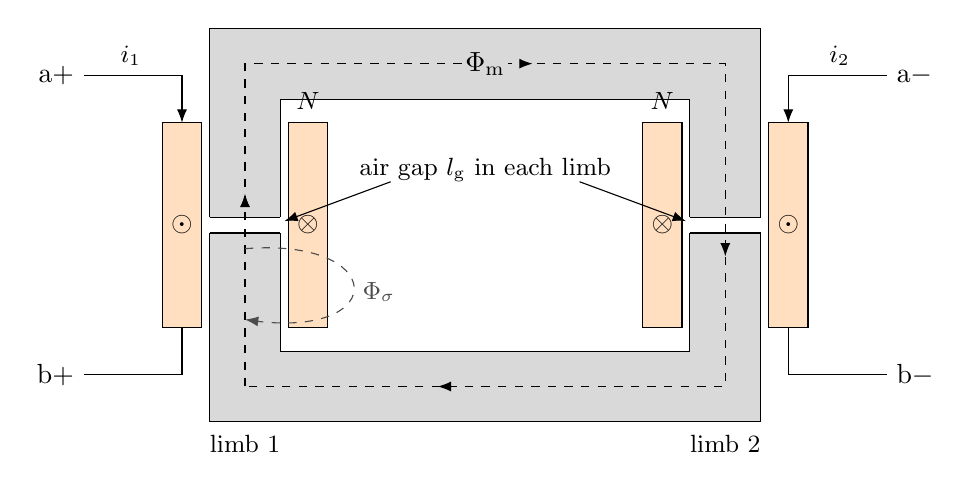
\begin{tikzpicture}[>=Latex, scale=1.0,
  fluxarrow/.style={dashed, postaction={decorate},
    decoration={markings,
      mark=at position 0.12 with {\arrow{>}},
      mark=at position 0.38 with {\arrow{>}},
      mark=at position 0.62 with {\arrow{>}},
      mark=at position 0.88 with {\arrow{>}}}}]
  % core (window type), limb/yoke thickness 0.9
  \fill[gray!30, even odd rule] (0,0) rectangle (7,5) (0.9,0.9) rectangle (6.1,4.1);
  \draw (0,0) rectangle (7,5);
  \draw (0.9,0.9) rectangle (6.1,4.1);
  % air gaps
  \fill[white] (-0.01,2.4) rectangle (0.91,2.6);
  \draw (0,2.4) -- (0.9,2.4) (0,2.6) -- (0.9,2.6);
  \fill[white] (6.09,2.4) rectangle (7.01,2.6);
  \draw (6.1,2.4) -- (7,2.4) (6.1,2.6) -- (7,2.6);
  % main flux loop (clockwise)
  \draw[fluxarrow] (0.45,0.45) -- (0.45,4.55) -- (6.55,4.55) -- (6.55,0.45) -- cycle;
  \node[fill=gray!30, inner sep=1pt] at (3.5,4.55) {$\Phi_\mathrm{m}$};
  % coil 1 sides (cross-section)
  \fill[orange!25] (-0.6,1.2) rectangle (-0.1,3.8);
  \fill[orange!25] (1.0,1.2) rectangle (1.5,3.8);
  \draw (-0.6,1.2) rectangle (-0.1,3.8);
  \draw (1.0,1.2) rectangle (1.5,3.8);
  \node at (-0.35,2.5) {$\odot$};
  \node at (1.25,2.5) {$\otimes$};
  \node[font=\small, above] at (1.25,3.85) {$N$};
  \node[font=\small, below] at (0.45,-0.05) {limb 1};
  % coil 2 sides
  \fill[orange!25] (5.5,1.2) rectangle (6.0,3.8);
  \fill[orange!25] (7.1,1.2) rectangle (7.6,3.8);
  \draw (5.5,1.2) rectangle (6.0,3.8);
  \draw (7.1,1.2) rectangle (7.6,3.8);
  \node at (5.75,2.5) {$\otimes$};
  \node at (7.35,2.5) {$\odot$};
  \node[font=\small, above] at (5.75,3.85) {$N$};
  \node[font=\small, below] at (6.55,-0.05) {limb 2};
  % leakage flux of coil 1 (lower part, through the window)
  \draw[dashed, gray!60!black, ->] (0.45,2.2) .. controls (2.3,2.35) and (2.3,1.0) .. (0.45,1.3);
  \node[gray!60!black, font=\small] at (2.15,1.65) {$\Phi_\sigma$};
  % terminals coil 1
  \draw[->] (-1.6,4.4) node[left] {a$+$} -- (-0.35,4.4) -- (-0.35,3.8);
  \node[font=\small, above] at (-1.0,4.4) {$i_1$};
  \draw (-0.35,1.2) -- (-0.35,0.6) -- (-1.6,0.6) node[left] {b$+$};
  % terminals coil 2
  \draw[->] (8.6,4.4) node[right] {a$-$} -- (7.35,4.4) -- (7.35,3.8);
  \node[font=\small, above] at (8.0,4.4) {$i_2$};
  \draw (7.35,1.2) -- (7.35,0.6) -- (8.6,0.6) node[right] {b$-$};
  % gap label
  \node[font=\small] at (3.5,3.2) {air gap $l_\mathrm{g}$ in each limb};
  \draw[->, thin] (2.3,3.05) -- (0.95,2.55);
  \draw[->, thin] (4.7,3.05) -- (6.05,2.55);
\end{tikzpicture}
\caption{Two-limb reactor: one coil per limb, air gap in each limb. The current symbols
($\odot$ out of the page, $\otimes$ into the page) are drawn for the load current,
$i_1 > 0$ and $i_2 < 0$: both coils drive the main flux $\Phi_\mathrm{m}$ in the same
direction around the core. $\Phi_\sigma$ is the leakage flux of coil~1, closing through
the window and not linking coil~2.}
\label{fig:core}
\end{figure}

The winding sense is chosen so that the load current magnetises the core: the
magnetomotive force along the main loop is
\begin{equation}
  \mathcal{F} = N i_1 - N i_2 = 2N\, i_\mathrm{m}, \qquad
  i_\mathrm{m} = \frac{i_1 - i_2}{2},
  \label{eq:im}
\end{equation}
where $i_\mathrm{m}$ is the magnetising current. For the load current, $i_1 = -i_2 = i$,
$i_\mathrm{m} = i$; for a common-mode current, $i_1 = i_2$, $i_\mathrm{m} = 0$ and the
core carries no main flux.

Two flux paths are considered. The main path, with reluctance $\mathcal{R}_\mathrm{m}$
(air gaps plus iron), links both coils:
\begin{equation}
  \Phi_\mathrm{m} = \frac{2N\, i_\mathrm{m}}{\mathcal{R}_\mathrm{m}} .
\end{equation}
The leakage path of each coil, with reluctance $\mathcal{R}_\sigma$ (air only), links
that coil alone. The flux linkages of the two coils are then
\begin{equation}
  \lambda_1 = \frac{L_\mathrm{d}}{2}\, i_1 + \frac{\psi}{2}, \qquad
  \lambda_2 = \frac{L_\mathrm{d}}{2}\, i_2 - \frac{\psi}{2},
  \label{eq:lambda}
\end{equation}
with
\begin{equation}
  \psi = 2N\Phi_\mathrm{m} = \frac{4N^2}{\mathcal{R}_\mathrm{m}}\, i_\mathrm{m} = L\, i_\mathrm{m},
  \qquad
  \frac{L_\mathrm{d}}{2} = \frac{N^2}{\mathcal{R}_\sigma} .
  \label{eq:LLd}
\end{equation}
$\psi$ is the flux linkage of the main path for the whole loop (both coils in series),
$L = 4N^2/\mathcal{R}_\mathrm{m}$ is the main inductance seen by the load current and
$L_\mathrm{d}$ the total leakage inductance seen by the load current. The sign of
$\psi/2$ in $\lambda_2$ follows from the winding sense of coil~2 and from the reference
direction of $i_2$ (a$-$ to b$-$). $L$, $L_\mathrm{d}$ and the winding resistance $R$
are the block parameters; they are \emph{total} values, and half of each is assigned to
each conductor.

\subsection{Voltage equations}

With $R/2$ per coil and the saturation model of Sec.~\ref{sec:sat}, which replaces
$\psi = L i_\mathrm{m}$ by $\mathrm{d}\psi = L\, k_L(i_\mathrm{m})\, \mathrm{d}i_\mathrm{m}$,
the terminal voltages $u_1$ (from a$+$ to b$+$) and $u_2$ (from a$-$ to b$-$) are
\begin{align}
  u_1 &= \frac{R}{2}\, i_1 + \frac{L_\mathrm{d}}{2}\, \frac{\mathrm{d}i_1}{\mathrm{d}t}
        + \frac{1}{2}\, \frac{\mathrm{d}\psi}{\mathrm{d}t}, \label{eq:u1}\\
  u_2 &= \frac{R}{2}\, i_2 + \frac{L_\mathrm{d}}{2}\, \frac{\mathrm{d}i_2}{\mathrm{d}t}
        - \frac{1}{2}\, \frac{\mathrm{d}\psi}{\mathrm{d}t}, \label{eq:u2}\\
  \frac{\mathrm{d}\psi}{\mathrm{d}t} &= L\, k_L(i_\mathrm{m})\, \frac{\mathrm{d}i_\mathrm{m}}{\mathrm{d}t}
        = L\, k_L(i_\mathrm{m})\, \frac{1}{2}\left(\frac{\mathrm{d}i_1}{\mathrm{d}t}
        - \frac{\mathrm{d}i_2}{\mathrm{d}t}\right). \label{eq:psi}
\end{align}
These three equations are what the block implements. Fig.~\ref{fig:circuit} shows the
equivalent circuit: each conductor carries $R/2$, the uncoupled leakage $L_\mathrm{d}/2$
and one half of the coupled (saturable) part.

\begin{figure}[htbp]
\centering
\begin{circuitikz}[european, scale=1.1, transform shape]
  \ctikzset{voltage dir=EF, inductor=american}
  \draw (0,3.6) node[left] {a$+$} to[short, i=$i_1$] (1.3,3.6)
        to[R, l=$R/2$] (3.1,3.6)
        to[L, l=$L_\mathrm{d}/2$] (4.9,3.6)
        to[L, l=$L/4$, name=Lone] (6.7,3.6)
        to[short] (8.0,3.6) node[right] {b$+$};
  \draw (0,0) node[left] {a$-$} to[short, i=$i_2$] (1.3,0)
        to[R, l_=$R/2$] (3.1,0)
        to[L, l_=$L_\mathrm{d}/2$] (4.9,0)
        to[L, l_=$L/4$, name=Ltwo] (6.7,0)
        to[short] (8.0,0) node[right] {b$-$};
  % coupling dots: a+ side of L1, b- side of L2
  \fill (Lone.west) ++(0.1,0.35) circle (2pt);
  \fill (Ltwo.east) ++(0.05,-0.42) circle (2pt);
  \draw[<->] (5.8,2.5) -- (5.8,1.1) node[midway, right] {$M = L/4$};
  % voltages, DIN convention: arrow from + to -
  \draw[->] (0.7,2.95) -- (7.3,2.95) node[midway, below] {$u_1$};
  \draw[->] (0.7,-0.95) -- (7.3,-0.95) node[midway, below] {$u_2$};
  \draw[dashed, gray] (-0.2,-1.6) rectangle (8.2,4.6);
\end{circuitikz}
\caption{Equivalent circuit of the block in the linear region. The dots mark the
coupling: with both currents referred from a to b, the mutual term is $-M$; for the load
current ($i_1 = -i_2$) the coupled parts add up. Voltage arrows according to the DIN
convention (from higher to lower potential).}
\label{fig:circuit}
\end{figure}

\subsection{Differential-mode and common-mode behaviour}

With the mode currents and voltages
\begin{equation}
  i_\mathrm{d} = i_\mathrm{m} = \frac{i_1 - i_2}{2}, \quad
  i_\mathrm{c} = \frac{i_1 + i_2}{2}, \qquad
  u_\mathrm{d} = u_1 - u_2, \quad
  u_\mathrm{c} = \frac{u_1 + u_2}{2},
\end{equation}
eqs.~\eqref{eq:u1}--\eqref{eq:psi} separate into
\begin{align}
  u_\mathrm{d} &= R\, i_\mathrm{d} + \bigl[L_\mathrm{d} + L\, k_L(i_\mathrm{d})\bigr]
                  \frac{\mathrm{d}i_\mathrm{d}}{\mathrm{d}t}, \label{eq:dm}\\
  u_\mathrm{c} &= \frac{R}{2}\, i_\mathrm{c} + \frac{L_\mathrm{d}}{2}\,
                  \frac{\mathrm{d}i_\mathrm{c}}{\mathrm{d}t}. \label{eq:cm}
\end{align}
The differential mode is the single-phase inductor with saturation; the common mode sees
only $R/2$ and $L_\mathrm{d}/2$ per conductor and is linear. The two modes are decoupled
for any operating point: a common-mode current does not change the saturation state, and
saturation does not change the common-mode impedance (within the assumptions of
Sec.~\ref{sec:lim}).

\subsection{Coupled-inductor form}

Eqs.~\eqref{eq:u1}--\eqref{eq:psi} can be written with an inductance matrix,
\begin{equation}
  \begin{bmatrix} u_1 - \tfrac{R}{2} i_1 \\[1mm] u_2 - \tfrac{R}{2} i_2 \end{bmatrix}
  =
  \begin{bmatrix}
    \dfrac{L_\mathrm{d}}{2} + \dfrac{L\,k_L}{4} & -\dfrac{L\,k_L}{4} \\[3mm]
    -\dfrac{L\,k_L}{4} & \dfrac{L_\mathrm{d}}{2} + \dfrac{L\,k_L}{4}
  \end{bmatrix}
  \frac{\mathrm{d}}{\mathrm{d}t}
  \begin{bmatrix} i_1 \\[1mm] i_2 \end{bmatrix},
  \label{eq:matrix}
\end{equation}
i.e. two coupled inductors with (linear region, $k_L = 1$)
\begin{equation}
  L_1 = L_2 = \frac{L_\mathrm{d}}{2} + \frac{L}{4}, \qquad
  M = \frac{L}{4}, \qquad
  k = \frac{M}{\sqrt{L_1 L_2}} = \frac{L}{L + 2L_\mathrm{d}} .
\end{equation}
The negative sign of the off-diagonal terms is due to the reference directions (both
currents from a to b); with the dots of Fig.~\ref{fig:circuit} the coupling is positive
for the load current. The series-aiding inductance $L_1 + L_2 + 2M = L + L_\mathrm{d}$
is the inductance seen by the load current, the series-opposing inductance
$L_1 + L_2 - 2M = L_\mathrm{d}$ is the inductance seen by a common-mode current flowing
through both conductors in series. With the default parameters
($L = \SI{300}{\micro\henry}$, $L_\mathrm{d} = \SI{20}{\micro\henry}$):
$L_1 = L_2 = \SI{85}{\micro\henry}$, $M = \SI{75}{\micro\henry}$, $k = 0.882$.
Saturation scales the coupled part only: $L/4$ and $M$ become $k_L L/4$, the leakage
$L_\mathrm{d}/2$ is unchanged.

The determinant of the matrix in \eqref{eq:matrix} is
$\tfrac{L_\mathrm{d}}{2}\bigl(\tfrac{L_\mathrm{d}}{2} + \tfrac{L\,k_L}{2}\bigr)$, positive
for $L_\mathrm{d} > 0$: the two currents are then independent states. With
$L_\mathrm{d} = 0$ the common-mode current would have no inductance and would be fixed
algebraically by the external network; the block therefore requires $L_\mathrm{d} > 0$.

\section{Saturation characteristic}
\label{sec:sat}

\subsection{Differential inductance table}

The saturation is described by the differential (incremental) inductance of the main
path, normalised to $L$,
\begin{equation}
  k_L(i_\mathrm{m}) = \frac{1}{L}\, \frac{\mathrm{d}\psi}{\mathrm{d}i_\mathrm{m}},
  \qquad
  x = \frac{|i_\mathrm{m}|}{\sqrt{2}\, I_\mathrm{base}},
\end{equation}
as a function of the magnetising current normalised to the peak value of the base
current $I_\mathrm{base}$ (rms). The table is the same as in the single-phase block
(Table~\ref{tab:sat}); it is stored as private parameters of the component and is
interpolated linearly, with nearest-value extrapolation ($k_L = 0.39$ beyond
$x = 3.85$). The characteristic is applied to the magnetising current, i.e.\ to the net
magnetomotive force of the core, not to the individual winding currents.

\begin{table}[htbp]
\centering
\caption{Saturation table (private parameters \texttt{Normalized\_current},
\texttt{L\_saturation}) and normalised flux linkage of the main path
$\Psi_\mathrm{n}(x) = \int_0^x k_L\,\mathrm{d}\xi$ at the breakpoints.}
\label{tab:sat}
\begin{tabular}{@{}S[table-format=1.2]S[table-format=1.2]S[table-format=1.3]S[table-format=1.3]@{}}
\toprule
{$x$} & {$k_L$} & {$\Psi_\mathrm{n}$} & {$\Psi_\mathrm{n}/x$} \\
\midrule
0    & 1.00 & 0     & 1.000 \\
1.00 & 1.00 & 1.000 & 1.000 \\
1.35 & 1.00 & 1.350 & 1.000 \\
2.30 & 0.88 & 2.243 & 0.975 \\
3.85 & 0.39 & 3.227 & 0.838 \\
\bottomrule
\end{tabular}
\end{table}

\subsection{Flux linkage}

The flux linkage of the main path follows by integration of the table,
\begin{equation}
  \psi(i_\mathrm{m}) = \operatorname{sgn}(i_\mathrm{m})\, L\, \sqrt{2}\, I_\mathrm{base}\,
  \Psi_\mathrm{n}(x), \qquad
  \Psi_\mathrm{n}(x) = \int_0^x k_L(\xi)\, \mathrm{d}\xi ,
\end{equation}
which is piecewise quadratic and continuous with its first derivative
(Fig.~\ref{fig:sat}). The total flux linkage seen by the load current, including the
leakage, is
\begin{equation}
  \psi_\mathrm{tot} = L_\mathrm{d}\, i_\mathrm{m} + \psi(i_\mathrm{m}),
  \label{eq:psitot}
\end{equation}
and is the quantity available at the \texttt{psi} output of the block (the same as the
\texttt{psi} output of the single-phase block).

Note that the table describes the \emph{differential} inductance. The apparent
(secant) inductance $\psi/i_\mathrm{m} = L\,\Psi_\mathrm{n}(x)/x$ decreases much less
(Table~\ref{tab:sat}: \SI{84}{\percent} at $x = 3.85$, where the differential
inductance is at \SI{39}{\percent}). When the table is filled from manufacturer data,
check which of the two the data sheet gives: small-signal measurements at DC bias give
the differential inductance, $V/(\omega I)$ measurements at rated AC current give a
value close to the apparent one.

\begin{figure}[htbp]
\centering
\begin{tikzpicture}
\begin{axis}[
  width=0.48\textwidth, height=5.2cm,
  xlabel={$x = |i_\mathrm{m}|/(\sqrt{2}\,I_\mathrm{base})$},
  ylabel={$k_L$},
  xmin=0, xmax=4.5, ymin=0, ymax=1.1,
  grid=major, grid style={gray!30},
  title={(a) differential inductance},
  title style={font=\small}, label style={font=\small}, tick label style={font=\small}]
  \addplot[blue, thick, mark=*, mark size=1.6pt] table[x=x, y=kL] {\tabkL};
\end{axis}
\end{tikzpicture}
\hfill
\begin{tikzpicture}
\begin{axis}[
  width=0.48\textwidth, height=5.2cm,
  xlabel={$x = |i_\mathrm{m}|/(\sqrt{2}\,I_\mathrm{base})$},
  ylabel={$\Psi_\mathrm{n}$},
  xmin=0, xmax=4.5, ymin=0, ymax=4.5,
  grid=major, grid style={gray!30},
  title={(b) flux linkage of the main path},
  title style={font=\small}, label style={font=\small}, tick label style={font=\small},
  legend pos=north west, legend style={font=\small, draw=none, fill=none}]
  \addplot[blue, thick] table[x=x, y=psi] {\tabpsi};
  \addlegendentry{$\Psi_\mathrm{n}(x)$}
  \addplot[gray, dashed] coordinates {(0,0) (4.5,4.5)};
  \addlegendentry{no saturation}
\end{axis}
\end{tikzpicture}
\caption{Saturation characteristic with the default table: (a) normalised differential
inductance $k_L$ (linear interpolation, nearest-value extrapolation beyond $x = 3.85$);
(b) normalised flux linkage of the main path $\Psi_\mathrm{n}$, obtained by integration
of (a).}
\label{fig:sat}
\end{figure}

Setting $I_\mathrm{base} = \infty$ gives $x = 0$ and $k_L = 1$ for any current, which
disables the saturation.

\section{Relation with the single-phase block}
\label{sec:equiv}

For $i_1 = -i_2 = i$, eqs.~\eqref{eq:u1}--\eqref{eq:psi} give
\begin{equation}
  u_1 - u_2 = R\, i + \bigl[L_\mathrm{d} + L\, k_L(i)\bigr] \frac{\mathrm{d}i}{\mathrm{d}t},
  \qquad
  \psi_\mathrm{tot} = L_\mathrm{d}\, i + \int L\, k_L(i)\, \mathrm{d}i ,
\end{equation}
which are exactly the equations of \texttt{singlephase\_inductor\_with\_saturation}
with the same $L$, $L_\mathrm{d}$, $R$ and $I_\mathrm{base}$. The two-limb block can
therefore replace the single-phase block in a two-wire circuit without changing the
parameters: the load current sees the same impedance and the same saturation, the
voltage drop is split evenly between the two conductors, and in addition the
common-mode path is represented by eq.~\eqref{eq:cm}.

\section{Simscape implementation}
\label{sec:impl}

\subsection{Interface}

Table~\ref{tab:if} lists the ports, the parameters and the outputs of the component.
The port labels a$+$ and a$-$ are on the left of the block, b$+$ and b$-$ on the right;
the physical-signal outputs are on the right.

\begin{table}[htbp]
\centering
\caption{Interface of \texttt{twolimb\_inductor\_with\_saturation}.}
\label{tab:if}
\begin{tabular}{@{}llll@{}}
\toprule
Item & Name & Default & Description \\
\midrule
node & \texttt{ap} (a$+$) & & winding 1, a side \\
node & \texttt{bp} (b$+$) & & winding 1, b side \\
node & \texttt{an} (a$-$) & & winding 2, a side \\
node & \texttt{bn} (b$-$) & & winding 2, b side \\
\midrule
parameter & \texttt{L} & \SI{300}{\micro\henry} & main inductance $L$, total (linear region) \\
parameter & \texttt{Ld} & \SI{20}{\micro\henry} & leakage inductance $L_\mathrm{d}$, total \\
parameter & \texttt{R} & \SI{2.4}{\milli\ohm} & winding resistance $R$, total \\
parameter & \texttt{i\_base} & \SI{360}{\ampere} (rms) & base current $I_\mathrm{base}$ of the saturation table \\
\midrule
output & \texttt{psi} & \si{\volt\second} & total flux linkage $\psi_\mathrm{tot}$, eq.~\eqref{eq:psitot} \\
output & \texttt{im} & \si{\ampere} & magnetising current $i_\mathrm{m}$, eq.~\eqref{eq:im} \\
\bottomrule
\end{tabular}
\end{table}

\subsection{Variables, equations and states}

The component declares the branch currents $i_1$ (\texttt{ap} $\to$ \texttt{bp}) and
$i_2$ (\texttt{an} $\to$ \texttt{bn}), the branch voltages $u_1$, $u_2$, the algebraic
variables $i_\mathrm{m}$, $x$ (\texttt{i\_norm}) and $k_L$ (\texttt{kL}), and the flux
linkage $\psi$ of the main path. The equations are \eqref{eq:im}, the table lookup,
\eqref{eq:psi}, \eqref{eq:u1} and \eqref{eq:u2}, plus the two output equations: ten
equations for eight variables and two outputs.

Three variables appear differentiated, $i_1$, $i_2$ and $\psi$. The two currents are the
physical states, with the mass matrix of eq.~\eqref{eq:matrix}. $\psi$ is a pure
integrator of $L\,k_L\,\mathrm{d}i_\mathrm{m}/\mathrm{d}t$, used only for the
\texttt{psi} output; its initial value is $0$ with high priority, which is consistent
with zero initial current. If the network imposes a non-zero initial current, $\psi$
starts with an offset equal to $\psi(i_\mathrm{m}(0))$; this affects the output only, not
the dynamics. $k_L$ is algebraic and carries no initial-value priority (a high-priority
target on an algebraic variable produces an initialisation warning whenever the initial
current is above $\sqrt{2}\,I_\mathrm{base}$).

The magnetising current enters the table through $|i_\mathrm{m}|$, which introduces a
zero crossing at $i_\mathrm{m} = 0$. It has no numerical consequence because $k_L$ is
flat ($k_L = 1$) up to $x = 1$; a symmetric table without the absolute value would avoid
the zero crossing at the cost of duplicating the table.

Parameter checks (\texttt{assert}) require $L > 0$, $L_\mathrm{d} > 0$, $R \ge 0$ and
$I_\mathrm{base} > 0$.

\subsection{Use}

The component is a plain \texttt{.ssc} file; it is used either inside a package folder
with \texttt{ssc\_build}, as the other components of the library, or through a
\emph{Simscape Component} block pointing at the file. The saturation table is stored as
private parameters, so a reactor with a different characteristic needs a copy of the
file with the two vectors edited; the breakpoints must be increasing and start at
$x = 0$.

The same file describes a common-mode choke by reversing the sense of coil~2: replace
$i_\mathrm{m} = (i_1 - i_2)/2$ with $(i_1 + i_2)/2$ and the sign of
$\tfrac{1}{2}\,\mathrm{d}\psi/\mathrm{d}t$ in eq.~\eqref{eq:u2}. The common-mode
current then magnetises the core and the load current sees the leakage only.

\section{Verification of the equations}
\label{sec:ver}

The equations \eqref{eq:im}--\eqref{eq:psi} were integrated numerically (variable-step
solver, relative tolerance $10^{-9}$), independently of Simscape, together with the
single-phase equation \eqref{eq:dm}, in the following test network: the terminals a$+$
and a$-$ are driven by ideal sources referred to ground,
$v_{\mathrm{a}+} = v_\mathrm{c} + v_\mathrm{d}/2$ and
$v_{\mathrm{a}-} = v_\mathrm{c} - v_\mathrm{d}/2$; the terminals b$+$ and b$-$ are loaded
by $R_\ell = \SI{0.1}{\ohm}$ each to ground. $v_\mathrm{d}$ is a \SI{50}{\hertz}
sinusoid of \SI{400}{\volt} peak, which drives the load current to $3.7$ p.u.\ ($k_L$
down to $0.45$); $v_\mathrm{c}$ is a \SI{1}{\kilo\hertz} sinusoid of \SI{20}{\volt}
peak, which drives a common-mode current of \SI{168}{\ampere} peak. Parameters at their
default values.

Fig.~\ref{fig:test} shows the steady-state waveforms. The results confirm the properties
of Sec.~\ref{sec:phys}:
\begin{itemize}
  \item the magnetising current $i_\mathrm{m}$ of the two-limb model coincides with the
        current of the single-phase model in the same differential-mode loop within
        \num{1e-4}~\si{\ampere} (peak \SI{1864}{\ampere}), and the \texttt{psi} outputs
        coincide within \num{1e-7}~\si{\volt\second};
  \item the common-mode current $i_\mathrm{c}$ follows eq.~\eqref{eq:cm} with the
        external $R_\ell$ within \num{2e-7}~\si{\ampere}; its amplitude
        $v_\mathrm{c}/\sqrt{(R_\ell + R/2)^2 + (\omega L_\mathrm{d}/2)^2} = \SI{168}{\ampere}$
        is unaffected by the saturation of the differential mode;
  \item the main-path flux linkage $\psi$ does not respond to $v_\mathrm{c}$.
\end{itemize}
The check validates the equations and the mode decoupling, not the Simscape syntax: the
\texttt{.ssc} file was not compiled in the environment in which this note was written
and must be built and tested in MATLAB, for instance with the same test network.

\begin{figure}[htbp]
\centering
\begin{tikzpicture}
\begin{axis}[
  width=0.95\textwidth, height=5.0cm,
  xlabel={$t$ (\si{\milli\second})}, ylabel={(\si{\ampere})},
  xmin=20, xmax=40, ymin=-2300, ymax=2300,
  grid=major, grid style={gray!30},
  title={(a) winding currents}, title style={font=\small},
  label style={font=\small}, tick label style={font=\small},
  legend columns=-1,
  legend style={font=\small, draw=none, fill=none, at={(0.5,-0.38)}, anchor=north}]
  \addplot[blue, thick] table[x=t, y=i1] {\tabiw};
  \addlegendentry{$i_1$}
  \addplot[red, thick] table[x=t, y=i2] {\tabiw};
  \addlegendentry{$i_2$}
\end{axis}
\end{tikzpicture}

\vspace{4mm}
\begin{tikzpicture}
\begin{axis}[
  width=0.95\textwidth, height=5.0cm,
  xlabel={$t$ (\si{\milli\second})}, ylabel={(\si{\ampere})},
  xmin=20, xmax=40, ymin=-2300, ymax=2300,
  grid=major, grid style={gray!30},
  title={(b) mode currents}, title style={font=\small},
  label style={font=\small}, tick label style={font=\small},
  legend columns=-1,
  legend style={font=\small, draw=none, fill=none, at={(0.5,-0.38)}, anchor=north}]
  \addplot[blue, thick] table[x=t, y=im] {\tabim};
  \addlegendentry{$i_\mathrm{m}$ two-limb}
  \addplot[black, dashed] table[x=t, y=is] {\tabim};
  \addlegendentry{$i$ single-phase}
  \addplot[green!60!black, thick] table[x=t, y=ic] {\tabim};
  \addlegendentry{$i_\mathrm{c}$}
\end{axis}
\end{tikzpicture}
\caption{Test with simultaneous differential-mode (\SI{400}{\volt}, \SI{50}{\hertz})
and common-mode (\SI{20}{\volt}, \SI{1}{\kilo\hertz}) excitation, default parameters:
(a) winding currents $i_1$, $i_2$; (b) magnetising current $i_\mathrm{m}$ compared with
the current of the single-phase block in the same loop (curves overlap) and common-mode
current $i_\mathrm{c}$. Saturation ($x$ up to $3.7$) raises the peak of
$i_\mathrm{m}$ from \SI{1770}{\ampere} (linear inductor) to \SI{1864}{\ampere}.}
\label{fig:test}
\end{figure}

\section{Limitations}
\label{sec:lim}

\begin{itemize}
  \item A single saturation factor is computed from the net magnetomotive force: the
        model assumes the same flux in both limbs (series magnetic circuit). The local
        flux that each coil drives through its own limb when the currents are not
        balanced (common-mode or asymmetric currents) is not represented; with large
        common-mode currents one limb may saturate locally.
  \item Leakage and common-mode inductance are lumped in the single linear parameter
        $L_\mathrm{d}/2$ per coil. In a real two-limb reactor the common-mode inductance
        is not necessarily half of the differential-mode leakage.
  \item No core losses, no winding capacitances, no temperature dependence; $R$ is
        constant.
  \item The differential inductance is piecewise linear, so
        $\mathrm{d}i/\mathrm{d}t$ has kinks at the breakpoints; $\psi(i)$ is continuous
        with its first derivative.
  \item Beyond the last breakpoint $k_L$ is held constant ($0.39$); in deep saturation
        the differential inductance of a real reactor tends to the air-core value.
\end{itemize}

\begin{thebibliography}{9}
\bibitem{erickson} R.~W. Erickson and D. Maksimovi\'c, \emph{Fundamentals of Power
  Electronics}, 3rd ed. Cham, Switzerland: Springer, 2020, ch.~13--14 (magnetics,
  coupled inductors).
\bibitem{kazimierczuk} M.~K. Kazimierczuk, \emph{High-Frequency Magnetic Components},
  2nd ed. Chichester, U.K.: Wiley, 2014.
\bibitem{simscape} The MathWorks, Inc., \emph{Simscape Language Guide}, Natick, MA,
  USA. [Online]. Available: \url{https://www.mathworks.com/help/simscape/}
\end{thebibliography}

\appendix
\section{Source listing}
\label{app:src}

File \texttt{twolimb\_inductor\_with\_saturation.ssc} (MIT licence header omitted).

\begin{lstlisting}
% Revision history
%   Rev. 00  2026-09-18  first issue

component twolimb_inductor_with_saturation
% Two-limb inductor with saturation
%
% Single-phase reactor with one winding on each limb of a common core:
% winding 1 between a+ and b+, winding 2 between a- and b-. The windings
% are connected so that the load (differential-mode) current, entering at
% a+ and returning at a-, magnetises the core in the same direction. A
% common-mode current (same direction in both conductors) does not
% magnetise the core and only sees the leakage inductance.
%
% L, Ld and R are the TOTAL values seen by the load current
% (a+ -> b+ -> load -> b- -> a-); half of each is placed in each conductor.
% With i1 = -i2 the block is identical to singlephase_inductor_with_saturation
% with the same parameters.
%
% Equivalent coupled-inductor description (linear region):
%   L1 = L2 = Ld/2 + L/4,   M = L/4,   k = L/(L + 2*Ld)
% The saturation factor kL(im) scales the coupled part (L/4 and M) only,
% im = (i1 - i2)/2 being the magnetising current (= load current in
% differential mode). The saturation table is the DIFFERENTIAL inductance
% dpsi/di normalised to L, versus |im| normalised to the peak base current
% sqrt(2)*i_base.
%
% To disable the saturation effect set i_base to inf.

    nodes
        ap = foundation.electrical.electrical;      % a+:left
        an = foundation.electrical.electrical;      % a-:left
        bp = foundation.electrical.electrical;      % b+:right
        bn = foundation.electrical.electrical;      % b-:right
    end

    outputs
        psi_out = {0, 'V*s'};    % psi
        im_out  = {0, 'A'};      % im
    end

    parameters
        L      = {300e-6, 'H'};      % Main (magnetising) inductance, total
        Ld     = {20e-6,  'H'};      % Leakage inductance, total
        R      = {2.4e-3, 'Ohm'};    % Winding resistance, total
        i_base = {360,    'A'};      % Base current (Arms)
    end

    parameters(Access=private)
        % dpsi/di normalised to L, versus |im| / (sqrt(2)*i_base)
        L_saturation       = {[1.0, 1.0, 1.0, 0.88, 0.39], '1'};
        Normalized_current = {[0, 1.0, 1.35, 2.30, 3.85],  '1'};
    end

    variables
        u1 = {0, 'V'};           % u1 (a+ to b+)
        u2 = {0, 'V'};           % u2 (a- to b-)
        i1 = {0, 'A'};           % i1 (a+ -> b+)
        i2 = {0, 'A'};           % i2 (a- -> b-)
        im = {0, 'A'};           % magnetising current (i1 - i2)/2
        i_norm = {0, '1'};       % |im| in p.u. of the peak base current
        kL = {1, '1'};           % saturation factor
        % core flux linkage of the main path, total for the loop
        psi = {value = {0, 'V*s'}, priority = priority.high};
    end

    branches
        i1 : ap.i -> bp.i;
        i2 : an.i -> bn.i;
    end

    equations
        assert(L > 0,      'Main inductance must be positive');
        assert(Ld > 0,     'Leakage inductance must be positive');
        assert(R >= 0,     'Winding resistance must be non-negative');
        assert(i_base > 0, 'Base current must be positive');

        u1 == ap.v - bp.v;
        u2 == an.v - bn.v;

        im == (i1 - i2)/2;
        i_norm == abs(im)/(i_base*sqrt(2));
        kL == tablelookup(Normalized_current, L_saturation, i_norm, ...
            interpolation = linear, extrapolation = nearest);

        % core (coupled) flux linkage, total for the loop: dpsi = L*kL(im)*dim
        psi.der == L*kL*(i1.der - i2.der)/2;

        % half of the leakage, resistance and core EMF in each conductor
        u1 == (R/2)*i1 + (Ld/2)*i1.der + psi.der/2;
        u2 == (R/2)*i2 + (Ld/2)*i2.der - psi.der/2;

        % total flux linkage seen by the load current (same as the single-phase block)
        psi_out == psi + Ld*im;
        im_out  == im;
    end
end
\end{lstlisting}

\end{document}
